\documentclass[aspectratio=169]{beamer}
\usepackage[utf8]{inputenc}
\usepackage[T1]{fontenc}
\usepackage{lmodern}
\usepackage[english]{babel}
\usepackage{graphicx}
\usepackage{caption}
\usepackage{subfigure}
\usepackage[export]{adjustbox}
\usepackage{multirow}
\usepackage{booktabs}
\usetheme{Boadilla}
%\usetheme{default}


\usepackage[backend=bibtex]{biblatex}
\addbibresource{references}


\newcommand\blfootnote[1]{%
  \begingroup
  \renewcommand\thefootnote{}\footnote{#1}%
  \addtocounter{footnote}{-1}%
  \endgroup
}

\captionsetup{font=scriptsize,labelfont=scriptsize}

\AtBeginSection[]
{
    \begin{frame}
        \frametitle{Outline}
        \tableofcontents[currentsection]
    \end{frame}
}

\setbeamertemplate{footline}[frame number]
\setbeamertemplate{navigation symbols}{}
\setbeamertemplate{items}[square]
\setbeamertemplate{section in toc}[square]
%\setbeamertemplate{itemize items}[default]
%\setbeamertemplate{enumerate items}[default]


\title[COMPSTAT 2024]{Univariate Time Series Forecasting using Echo State Networks: An Empirical Application}
\subtitle{26th International Conference on Computational Statistics}
\author[Alexander Häußer]{Alexander Häußer \blfootnote{\tiny{\url{alexander.haeusser@wirtschaft.uni-giessen.de}}}}
\institute[]{Justus-Liebig-University Giessen \\ Faculty 02 - Economics and Business Studies \\ Chair of Statistics and Econometrics}
\date{August 27, 2024}



\begin{document}

\begin{frame}
\titlepage
\end{frame}

\begin{frame}
\frametitle{Outline}
\tableofcontents
\end{frame}


\section{Introduction}


\begin{frame}[t]{Background and Research Objectives}
    \begin{minipage}[t]{0.5\textwidth}
        \vspace{0pt}
        \textbf{Neural networks for forecasting}
        \begin{itemize}
            \item Advantages
            	\begin{itemize}
            		\item Non-linearity and flexibility
            		\item Pattern recognition and sequential learning
            		\item Scalability
            	\end{itemize}
			\item Disadvantages
				\begin{itemize}
					\item Complexity and interpretability
					\item Model selection and overfitting
					\item Stability and convergence	
					\item Training time
				\end{itemize}
        \end{itemize}
    \end{minipage}%
    \hfill
    \begin{minipage}[t]{0.5\textwidth}
        \vspace{0pt}
        \textbf{Research objectives}
        \begin{itemize}
        	\item Statistical methods are hard to beat?!
        	\item Develop algorithm for fast and fully automatic time series modeling and forecasting 						  using Echo State Networks (ESN)
        	\item Empirical analysis
        		\begin{itemize}
        			\item Data from the M4 Forecasting Competition
        			\item Evaluate accuracy of (point) forecasts and measure computational run-time
        			\item Benchmark against state-of-the-art forecasting methods
        		\end{itemize}
        \end{itemize}
    \end{minipage}
\end{frame}





\section{Echo State Networks}



\begin{frame}[t]{Echo State Networks - Architecture}
    \begin{minipage}[t]{0.3\textwidth}
        \vspace{0pt}
        \begin{itemize}
			\item Input $u_{t} = y_{t-1}$ is non-linearly expanded into a high-dimensional feature space (i.e., internal states)
			\item Output $y_{t}$ is combined via trainable weights from these internal states
			\item Dashed lines indicate fixed weights and solid lines indicate trainable weights
        \end{itemize}
    \end{minipage}%
    \hfill
    \begin{minipage}[t]{0.7\textwidth}
        \vspace{0pt}
 		\begin{figure}[H]
		\center
			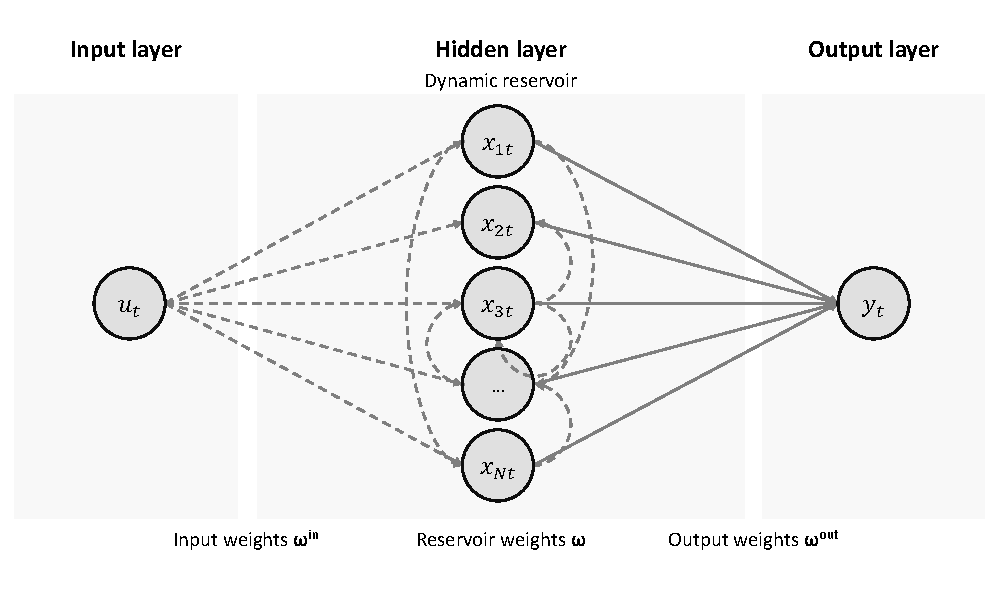
\includegraphics[scale=0.6]{figures/figure_04_architecture.pdf}
		\end{figure}
    \end{minipage}
\end{frame}







\begin{frame}[t]{Echo State Network - Basic model\footnote{More details in the Appendix}}
    \begin{minipage}[t]{0.33\textwidth}
        \vspace{0pt}
        \textbf{1. Data pre-processing}
        \begin{itemize}
            \item Identify non-stationarity via KPSS test
			\item If required, calculate (first) difference to remove non-stationarity
			\item Scale (stationary) time series to interval $[-0.5, 0.5]$
        \end{itemize}
    \end{minipage}%
    \hfill
    \begin{minipage}[t]{0.33\textwidth}
        \vspace{0pt}
        \textbf{2. Reservoir generation}
        \begin{itemize}
            \item Calculate the internal states (i.e., reservoir) according to
				\begin{equation*}
					\mathbf{x}_{t} = \tanh \left( {\boldsymbol{\omega}^{in}} u_{t} + \boldsymbol{\omega} \mathbf{x}_{t-1} \right)
				\end{equation*}
			\item First autoregressive lag as input, i.e., $u(t) = y(t-1)$
			\item Input and reservoir weight matrices $\boldsymbol{\omega}^{in}$ and $\boldsymbol{\omega}$
			\item Collect internal states in design matrix X
        \end{itemize}
    \end{minipage}
    \hfill
    \begin{minipage}[t]{0.33\textwidth}
        \vspace{0pt}
        \textbf{3. Model estimation and selection}
        \begin{itemize}
            \item Linear model
            	\begin{equation*}
            	\mathbf{y} = \mathbf{X} \boldsymbol{\omega}^{out} + \boldsymbol{\epsilon}
				\end{equation*}
			\item Estimate coefficients via ridge regression
				\begin{equation*}
				\boldsymbol{\hat{\omega}}^{out} = (\mathbf{X}^\top \mathbf{X} + \mathbf{R}_{\lambda})^{-1}\mathbf{X}^\top\mathbf{y}
				\end{equation*}
			\item Regularization parameter $\lambda$ is determined via random search by minimizing the BIC
        \end{itemize}
    \end{minipage}
\end{frame}




\begin{frame}[t]{Data from the M4 Forecasting Competition}
    \begin{minipage}[t]{0.3\textwidth}
        \vspace{0pt}
        \begin{itemize}
            \item Original M4 dataset consists of 100,000 time series
			\item Different frequencies and applications fields
			\item Randomly selected 2,400 monthly and 1,200 quarterly series
			\item Diverse dataset with different characteristics (trend, season, non-stationarity, etc.)
        \end{itemize}
    \end{minipage}%
    \hfill
    \begin{minipage}[t]{0.7\textwidth}
        \vspace{0pt}
 		\begin{figure}[H]
		\center
			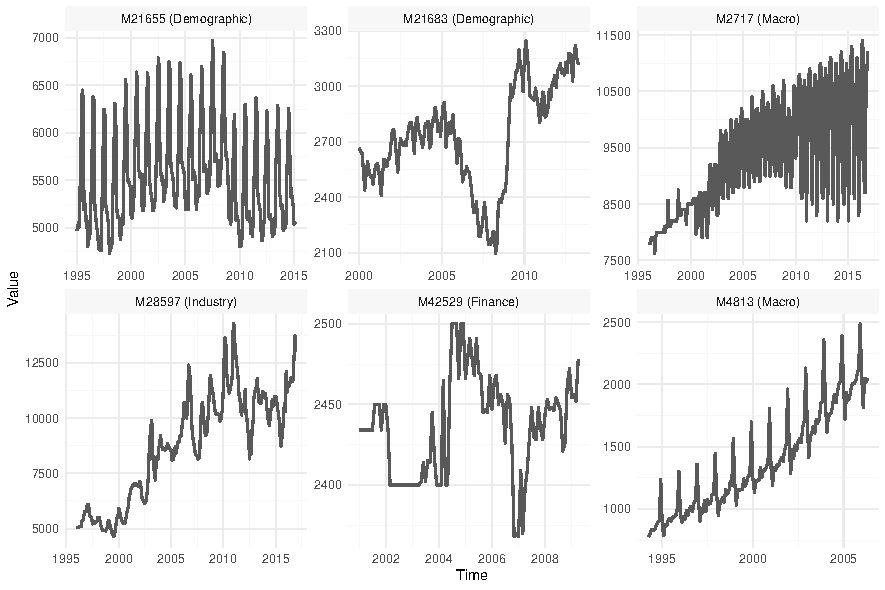
\includegraphics[scale=0.7]{figures/figure_03_data_sample_wide.pdf}
		\end{figure}
    \end{minipage}
\end{frame}



\begin{frame}[t]{Reservoir generation - Feature engineering using the echo state approach}
    \begin{minipage}[t]{0.3\textwidth}
        \vspace{0pt}
        \begin{itemize}
            \item Internal states (colored lines) and the pre-processed output variable (black line)
			\item Non-linear dimensionality expansion as a feature engineering technique for time series
			\item \textbf{Problem}: Multicollonearity and overfitting
        \end{itemize}
    \end{minipage}%
    \hfill
    \begin{minipage}[t]{0.7\textwidth}
        \vspace{0pt}
 		\begin{figure}[H]
		\center
			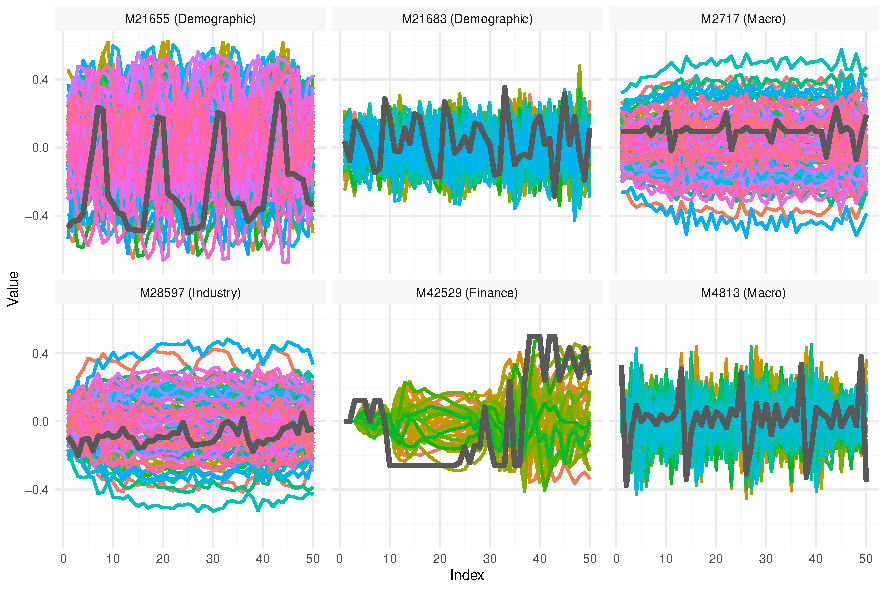
\includegraphics[scale=0.7]{figures/figure_05_model_states_wide.pdf}
		\end{figure}
    \end{minipage}
\end{frame}



\begin{frame}[t]{Model selection and estimation - Random search and ridge regression}
    \begin{minipage}[t]{0.3\textwidth}
        \vspace{0pt}
        \begin{itemize}
            \item Top 5 internal states (colored lines) and the pre-processed output variable (black line)
			\item Selection based on the size of the absolute value of the coefficients (high correlation $\rightarrow$ predictive power)
			\item Lead-lag relationship captures auto-correlation, seasonality, etc.
        \end{itemize}
    \end{minipage}%
    \hfill
    \begin{minipage}[t]{0.7\textwidth}
        \vspace{0pt}
 		\begin{figure}[H]
		\center
			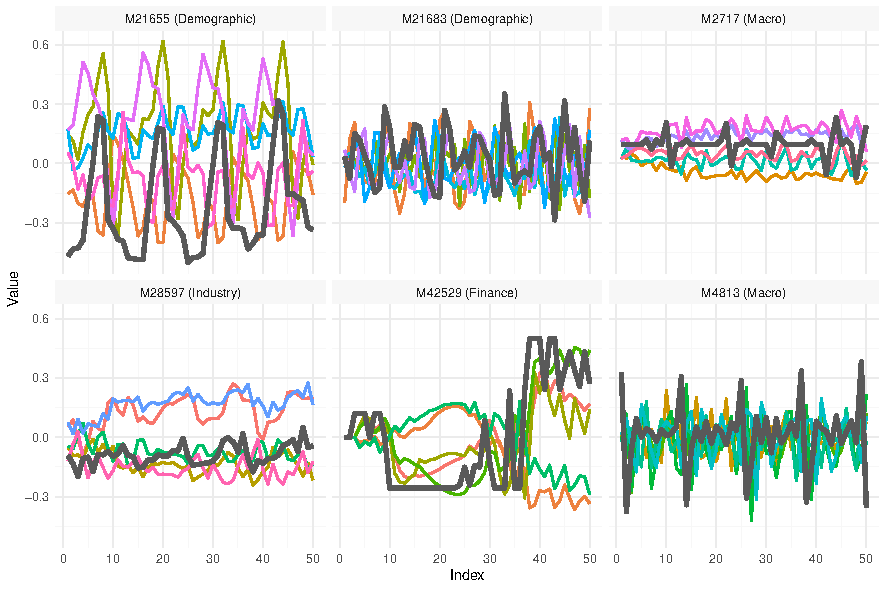
\includegraphics[scale=0.7]{figures/figure_06_model_states_top_wide.pdf}
		\end{figure}
    \end{minipage}
\end{frame}


\begin{frame}[t]{Actual values, fitted values and forecasts from trained ESN}
    \begin{minipage}[t]{0.3\textwidth}
        \vspace{0pt}
        \begin{itemize}
        	\item Recursive forecasting due to \textit{autoregressive nature}
            \item Actual values (black), fitted values (red) and out-of-sample forecasts (green)
			\item Vertical dotted line indicates the split of actual values into training and testing
			\item ESN model produces reasonable forecasts
        \end{itemize}
    \end{minipage}%
    \hfill
    \begin{minipage}[t]{0.7\textwidth}
        \vspace{0pt}
 		\begin{figure}[H]
		\center
			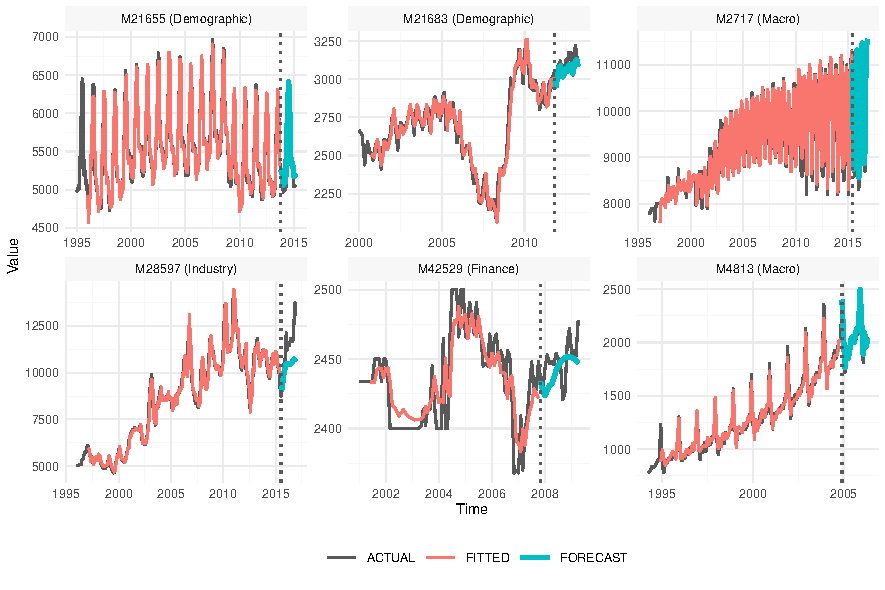
\includegraphics[scale=0.7]{figures/figure_07_model_forecast_sample_wide.pdf}
		\end{figure}
    \end{minipage}
\end{frame}



\section{Empirical application}

\begin{frame}[t]{Forecast Accuracy - Monthly dataset}
    \begin{minipage}[t]{0.3\textwidth}
        \vspace{0pt}
        \textbf{Key takeaways}
        \begin{itemize}
            \item ...
			\item ...
			\item ...
        \end{itemize}
    \end{minipage}%
    \hfill
    \begin{minipage}[t]{0.7\textwidth}
        \vspace{0pt}
 		\begin{table}[ht]
			\scriptsize
			\centering
			\begin{tabular}{lrrrrrr}
				\toprule
				\multirow{2}{*}{\textbf{Model}} & \multicolumn{2}{c}{\textbf{MASE}} & \multicolumn{2}{c}					{\textbf{sMAPE [\%]}} & \multicolumn{2}{c}{\textbf{Run Time [sec]}} \\
				\cmidrule(l){2-3} \cmidrule(l){4-5} \cmidrule(l){6-7}
 				& Mean & Median & Mean  & Median & Mean & Total \\
				\midrule
				ESN & \textbf{0.885} & 0.717 & 17.877 & 12.296 & 0.201 & 483.406 \\ 
				TBATS & 0.887 & \textbf{0.711} & 17.075 & 12.246 & 0.650 & 1561.136 \\ 
				ARIMA & 0.891 & 0.729 & 17.963 & 12.415 & 0.256 & 613.874 \\ 
				ETS & 0.902 & 0.722 & 17.763 & \textbf{12.182} & 0.167 & 401.617 \\ 
				THETA & 0.902 & 0.716 & \textbf{16.814} & 12.196 & 0.024 & 58.558 \\ 
				ELM & 0.930 & 0.739 & 18.430 & 13.081 & 23.995 & 57588.779 \\ 
				MLP & 1.026 & 0.839 & 21.398 & 14.637 & 2.209 & 5302.472 \\ 
				NNETAR & 1.042 & 0.830 & 19.663 & 14.374 & 39.318 & 94363.406 \\ 
				DRIFT & 1.077 & 0.806 & 20.013 & 13.750 & 0.025 & 60.752 \\ 
				NAIVE & 1.097 & 0.847 & 19.573 & 14.419 & 0.030 & 72.308 \\ 
				PROPHET & 1.143 & 0.890 & 23.901 & 15.859 & 0.783 & 1879.991 \\ 
				SNAIVE & 1.165 & 0.948 & 20.489 & 15.770 & 0.025 & 60.429 \\ 
				TSLM & 1.538 & 1.156 & 31.740 & 20.203 & 0.030 & 71.990 \\ 
				MEDIAN & 2.841 & 1.788 & 37.020 & 31.912 & \textbf{0.024} & \textbf{56.925} \\ 
				MEAN & 2.849 & 1.958 & 38.178 & 33.766 & 0.026 & 61.436 \\ 
				\bottomrule
			\end{tabular}
		\end{table}
    \end{minipage}
\end{frame}




\begin{frame}[t]{Forecast Accuracy - Quarterly dataset}
    \begin{minipage}[t]{0.3\textwidth}
        \vspace{0pt}
        \textbf{Key takeaways}
        \begin{itemize}
            \item ...
			\item ...
			\item ...
        \end{itemize}
    \end{minipage}%
    \hfill
    \begin{minipage}[t]{0.7\textwidth}
        \vspace{0pt}
 		\begin{table}[ht]
			\scriptsize
			\centering
			\begin{tabular}{lrrrrrr}
				\toprule
				\multirow{2}{*}{\textbf{Model}} & \multicolumn{2}{c}{\textbf{MASE}} & \multicolumn{2}{c}					{\textbf{sMAPE [\%]}} & \multicolumn{2}{c}{\textbf{Run Time [sec]}} \\
				\cmidrule(l){2-3} \cmidrule(l){4-5} \cmidrule(l){6-7}
 				& Mean & Median & Mean  & Median & Mean & Total \\
				\midrule
				ETS & \textbf{1.082} & \textbf{0.839} & 10.264 & 5.398 & 0.062 & 74.100 \\ 
				TBATS & 1.104 & 0.843 & \textbf{9.975} & 5.579 & 0.336 & 403.254 \\ 
				ELM & 1.114 & 0.880 & 10.771 & \textbf{5.352} & 1.382 & 1658.841 \\ 
				ESN & 1.114 & 0.908 & 10.672 & 5.540 & 0.052 & 61.836 \\ 
				ARIMA & 1.119 & 0.876 & 10.410 & 5.703 & 0.106 & 127.593 \\ 
				THETA & 1.150 & 0.908 & 10.339 & 5.859 & 0.026 & 31.040 \\ 
				DRIFT & 1.155 & 0.888 & 10.915 & 5.524 & 0.025 & 30.375 \\ 
				MLP & 1.187 & 0.917 & 11.673 & 5.833 & 0.602 & 722.079 \\ 
				NAIVE & 1.329 & 1.070 & 11.358 & 6.813 & 0.035 & 41.978 \\ 
				PROPHET & 1.435 & 1.089 & 14.316 & 7.070 & 1.653 & 1983.211 \\ 
				NNETAR & 1.444 & 1.126 & 12.793 & 7.358 & 25.078 & 30093.072 \\ 
				SNAIVE & 1.513 & 1.282 & 12.753 & 8.003 & 0.025 & 29.628 \\ 
				TSLM & 1.879 & 1.478 & 16.222 & 9.759 & 0.028 & 33.849 \\ 
				MEAN & 4.241 & 3.567 & 29.691 & 24.863 & \textbf{0.024} & \textbf{28.402} \\ 
				MEDIAN & 4.361 & 3.510 & 31.259 & 24.729 & 0.024 & 29.179 \\ 
				\bottomrule
			\end{tabular}
		\end{table}
    \end{minipage}
\end{frame}



\section{Summary}


\begin{frame}[t]{Summary and concluding remarks}
    \begin{minipage}[t]{0.5\textwidth}
        \vspace{0pt}
        \textbf{Summary}
        \begin{itemize}
            \item Proposed model achieved high accuracy and can outperform or compete against state-of-the-art forecasting methods
            \item Empirical results demonstrate the universal learning capabilities and the potential of ESNs
            \begin{itemize}
            	\item Data-driven instead of model-driven forecasts
            	\item Being more generic and making less assumptions
            \end{itemize}
        \end{itemize}
    \end{minipage}%
    \hfill
    \begin{minipage}[t]{0.5\textwidth}
        \vspace{0pt}
        \textbf{Outlook}
        \begin{itemize}
        	\item Probabilistic forecasting, i.e., enhance point forecasts with forecast distributions
        	\item Multivariate forecasting and exogenous inputs
        	\item Reservoir generation as feature engineering technique
        \end{itemize}
    \end{minipage}
\end{frame}


\section{References}

\begin{frame}[allowframebreaks]
    \frametitle{References}
    \nocite{*}
    \printbibliography[heading=none]
\end{frame}

\section{Appendix}



\begin{frame}
\frametitle{Univariate Electricity Load Forecasting using ESNs}
\framesubtitle{\large Basic model (2/2)}

\begin{itemize}
\item Input: $\mathbf{u}_t = \{ u_{1,t}, u_{2,t},...,u_{K,t} \}$
\item Internal states (reservoir): $\mathbf{x}_t = \{ x_{1,t}, x_{2,t},...,x_{N,t} \}$
\item Output: $\mathbf{y}_t = \{ y_{1,t}, y_{2,t},...,y_{L,t} \}$
\end{itemize}

\begin{itemize}
\item Randomly generate input weight matrix $\mathbf{W}^{in} \in \mathbb{R}^{N \times K}$
\item Randomly generate reservoir weight matrix $\mathbf{W} \in \mathbb{R}^{N \times N}$ using the spectral radius $\rho$
\end{itemize}

\begin{subequations}
\begin{align}
\mathbf{\widetilde{x}}_{t} &= \tanh \left( {\mathbf{W}^{in}} \mathbf{u}_{t} + \mathbf{W}\mathbf{x}_{t - 1} \right), \label{eq:update} \\
\mathbf{x}_{t} &= (1 - \alpha )\mathbf{x}_{t - 1} + \alpha \mathbf{\widetilde{x}}_{t} \label{eq:states}
\end{align}
\end{subequations}

%\begin{equation}
%\mathbf{y}_{t} = \mathbf{W}^{out} \mathbf{x}_{t} + \boldsymbol{\epsilon}_{t},
%\label{eq:model}
%\end{equation}

\begin{itemize}
\item The output is defined as $\mathbf{y}_{t} = \mathbf{W}^{out} \mathbf{x}_{t} + \boldsymbol{\epsilon}_{t}$, which is a linear optimization problem. The readout weight matrix $\mathbf{W}^{out}$ is usually computed using ridge regression.
\end{itemize}

\end{frame}





\begin{frame}
\frametitle{Univariate Electricity Load Forecasting using ESNs}
\framesubtitle{\large Training via ridge regression and forecasting}

\begin{itemize}
\item Given the target output $y_{t}$ and the design matrix $\mathbf{x}_{t}$, the optimization problem is defined as the penalized residual sum of squares (PRSS):
\end{itemize}

\begin{subequations}
\begin{align}
PRSS(\mathbf{W}^{out})_{l_2} &= \sum\limits_{t = 1}^T {{{\left( {y_{t} - {\mathbf{x}_{t}^T}{\mathbf{W}^{out}}} \right)}^2}} + \lambda \sum\limits_{n = 1}^N {{{\left( {\mathbf{W}_n^{out}} \right)}^2}}, \\
&= \underbrace {{{\left( {\mathbf{y} - \mathbf{X}{\mathbf{W}^{out}}} \right)}^T}\left( {\mathbf{y} - \mathbf{X}{\mathbf{W}^{out}}} \right)}_{RSS} + \underbrace {\lambda \left\| {{\mathbf{W}^{out}}} \right\|_2^2}_{Penalty} \label{eq:problem}
\end{align}
\end{subequations}

\begin{itemize}
\item The solution to the ridge regression problem is given by
\end{itemize}

\begin{equation}
\mathbf{\hat{W}}^{Out} = (\mathbf{X}^T\mathbf{X} + \lambda\mathbf{I}_N)^{-1}\mathbf{X}^{T}\mathbf{y}.
\label{estimator}
\end{equation}

\end{frame}





\begin{frame}[t]{Echo State Network  - Settings and hyperparameters}
    \begin{minipage}[t]{0.5\textwidth}
        \vspace{0pt}
        \textbf{Reservoir generation}
        	\begin{table}[ht]
        	\scriptsize
			\centering
				\begin{tabular}{ll}
				\toprule
				\textbf{Setting}                                    & \textbf{Value}                   \\
				\midrule
				Input ($\mathbf{u}$)                                & $y_{t-1}$                        \\
				Output ($\mathbf{y}$)                               & $y_{t}$                          \\
				Activation function                                 & $tanh(.)$                        \\
				Internal states ($N$)                               & $min(\lfloor 0.4T \rfloor, 100)$ \\
				Initial drop-out ($\delta$)                         & $\lfloor 0.05T \rfloor$          \\
				\midrule
				Input weight matrix ($\boldsymbol{\omega}^{in}$)    &                                  \\
				\hspace{2.5mm} Dimension                            & $N \times 1$                     \\
				\hspace{2.5mm} Random uniform                       & $[-0.5, 0.5]$                    \\
				\hspace{2.5mm} Density                              & 100\%                            \\
				\midrule
				Reservoir weight matrix ($\boldsymbol{\omega}$)     &                                  \\
				\hspace{2.5mm} Dimension                            & $N \times N$                     \\
				\hspace{2.5mm} Random uniform                       & $[-0.5, 0.5]$                    \\
				\hspace{2.5mm} Density                              & 50\%                             \\
				\hspace{2.5mm} Spectral radius ($\rho$)             & $1.0$                            \\
				\bottomrule
				\end{tabular}
			\end{table}
    \end{minipage}%
    \hfill
    \begin{minipage}[t]{0.5\textwidth}
        \vspace{0pt}
        \textbf{Model estimation and selection}
        	\begin{table}[ht]
        	\scriptsize
			\centering
				\begin{tabular}{ll}
				\toprule
				\textbf{Setting}                                  & \textbf{Value}	 \\
				\midrule
				Model type                                        & Linear model	 \\
				Estimator                                         & Ridge regression \\
				Optimization algorithm                            & Random search 	 \\
				Search space ($\lambda$)                          &  				 \\
				\hspace{2.5mm} Number of random values ($K$)      & $2N$             \\
				\hspace{2.5mm} Interval of random uniform         & $[10^{-4}, 2]$   \\
				Information criterion                             & BIC              \\
				\bottomrule
				\end{tabular}
			\end{table}
    \end{minipage}
\end{frame}



\end{document}
